\chapter{Zweite Iteration}\label{chap:pro2}
In \autoref{subsec:test1} haben sich während der Testphase des ersten Prototyps sowohl neue Probleme als auch fehlende Funktionen identifizieren lassen.
Diese sollen bei der Entwicklung eines zweiten Prototyps in diesem Abschnitt berücksichtigt werden. 
Hierzu werden die vier Phasen des \hcdp{} ein weiteres Mal durchlaufen.

\section{Observation}
Um einen Überblick über die Test-Ergebnisse aus \autoref{subsec:test1} herzustellen, werden diese im Nachfolgenden zunächst noch einmal aufgelistet und anschließend weiter evaluiert:

\begin{itemize}
  \item Bedienung der App nicht intuitiv
  \item Text- und Formelemente auf Tablet-Geräten nicht gut bedienbar
  \item Eingetragene Messwerte bei dunklem Hintergründen nicht gut erkennbar
  \item Anwenderwunsch: Zuordnen von Gerüsttypen zu Formen
  \item Anwenderwunsch: Zuschneiden und Rotieren des Bildes
\end{itemize}

\noindent
Zunächst auffällig ist, dass beide Testpersonen in \autoref{subsec:test1} die \emph{Floating Action Buttons} als Hindernis bei der Bedienung der App beschreiben.
Da alle möglichen Aktionen erst dann sichtbar werden, wenn der \emph{Floating Action Button} angeklickt wird, und sonst nur ein einzelnes Icon angezeigt wird, wird dem Nutzer keine angemessene Rückmeldung über den aktuellen Systemzustand gegeben.
Außerdem wird hierdurch keine ausreichende Hilfestellung zu den vorhandenen Funktionen, und wie diese zu benutzen sind gegeben.
(Nielsen~\autoref{itm:N1} \& \autoref{itm:N10}) \\

Ein weiterer Punkt, der in \autoref{subsec:test1} negativ aufgefallen ist, ist die Benutzung der App auf Tablet-Geräten.
Damit Endgeräte mit einer großen Bildschirmdiagonale trotzdem über eine scharfe Auflösung verfügen, besitzen diese mehr Pixel pro Zentimeter bzw. eine höhere Pixeldichte.
Da die UI-Elemente im ersten Prototyp mit Hilfe von \emph{Pixeln}, welche von Android zur Laufzeit nicht für die entsprechenden Bildschirmgrößen optimiert werden, modelliert worden sind, werden UI-Elemente auf Tablet-Geräten kleiner dargestellt, als auf normalen Smartphones.
Dies erschwert die Benutzung der App auf Tablets, da Texte nur mühsam zu lesen, und Formen schwierig auszuwählen sind.
So werden hier einerseits potentielle Fehlerquellen generiert, andererseits wird das Nutzungerlebnis auf Tablet-Geräten negativ beeinflusst.
(Nielsen~\autoref{itm:N5} \& \autoref{itm:N13}) \\

Darüber hinaus zeigen die Testergebnisse, dass die Testpersonen Probleme beim Erkennen von eingetragenen Messwerten auf dunklen Bildern haben.
Die schlechte Lesbarkeit der Messwerte resultiert wahrscheinlich aus der grauen Textfarbe, welche unabhängig vom Farbraum des Bildes festgelegt ist.
Zudem fehlt ein Hintergrund, der unter dem Text liegt, und diesen so vom eigentlichen Bild abhebt.
(Nielsen~\autoref{itm:N12}). \\

Zusätzlich zu den Problemen, die während der Testphase des ersten Prototyps identifiziert worden sind, haben sich bei den Testpersonen Wünsche für Funktionen, die nicht in der Implementierung des ersten Prototyps zu finden sind, aber im Alltag regelmäßig benötigt werden, herauskristallisiert. 
So soll die \emph{Library} zum Einen um eine Funktionen erweitert werden, die es ermöglicht, eingetragene Formen mit vordefinierten Gerüsttypen zu verknüpfen.
Zum Anderen soll die Möglichkeit bestehen, Bilder beim Import in die App in die gewünschte Größe und Form schneiden zu können.

\section{Idea Generation}\label{sec:idea2}
\todo{refs auf papers/guidelines wie bei Konzeption}
Um dem Benutzer jederzeit eine klare und einfache Rückmeldung über den aktuellen Systemzustand und die darin ausführbaren Aktionen zu geben, bietet es sich an, eine Art Statusleiste am unteren Bildschirmrand zu verankern.
Diese soll mit Hilfe von unterscheidbaren, aber intuitiv verständlichen Icons, über den aktuellen Modus (Zeichnen oder Text) informieren, und zugleich nicht-benutzbare Aktionen nicht-auswählbar gestalten. \\
\todo{Worauf hier reffen?}

Für eine bessere und einfachere Benutzung der App auf Tablet-Geräten könnte eine zweite Benutzeroberfläche, die nur bei Geräten mit einer Displaybreite von beispielsweise mindestens $600$ Pixeln benutzt wird, in die App eingebunden werden. 
Alternativ besteht die Möglichkeit, die Größe diverser Text- und Formelemente mit der Bildschirmgröße zu skalieren.
Dies hat den Effekt, dass Bildschirm-Elemente bei verschiedenen Bildschirmgrößen immer ungefähr gleich groß sind.
\\
\todo{Supporting multiple screens android devguides}

Die schlechte Erkennbarkeit von eingetragenen Messwerten auf Bildern mit dunklem Hintergrund lässt sich durch das Anpassen der Textfarbe in Kombination mit der Benutzung eines Texthintergrundes lösen.
So könnte, wie bei \emph{Toasts}, die im Android System seit API X vorhanden sind, ein dunkler Hintergrund mit einem hellen Text dazu genutzt werden, eingetragene Messwerte unabhängig von den Lichtverhältnissen im Bild gut erkennbar zu gestalten. \\
\todo{ref auf toast}

Um Formen direkt den passenden Gerüsttypen zuzuordnen, bietet sich ein modaler Dialog an.
Dieser könnte zum Beispiel bei einem langen Klick auf die gewünschte Form angezeigt werden, und in einem \emph{Dropdown} vorhandene Gerüsttypen zur Auswahl anbieten.
Falls ein langer Klick auf die Form bei der ersten Benutzung zu kontraintuitiv ist, würde sich eine Option in der oben beschriebenen Statusleiste anbieten, die nur dann auswählbar ist, wenn zuvor eine Form markiert wurde.
Zudem muss an der From selbst erkenntlich werden, dass diese mit einem Gerüsttypen verlinkt ist. \\
\todo{Dropdowns und long press gestures}

Das Schneiden und Rotieren von Bildern kann einerseits durch die Benutzung der im Android-System vorhandenen \emph{Crop-Activity} realisiert werden, andererseits würde sich auch die Benutzung einer dedizierten \emph{Android-Library} für das Schneiden von Bildern anbieten.
Ersteres bringt die Gefahr mit sich, dass die Verfügbarkeit einer solchen \emph{Crop-Activity} im Android-System vom Gerätehersteller und der verwendeten Android-Version abhängig ist, sodass nicht sichergestellt werden kann, dass die Funktion auf allen Geräten funktionieren wird. \\
\todo{ref auf API docs}

\section{Prototyping}

Der zweite Prototyp wurde am 3. Januar 2018 fertiggestellt, und umfasst die Implementierung der in \autoref{subsec:idea2} gesammelten Ideen. \\

Die Statusleiste wurde durch eine \emph{Bottom-Bar} am unteren Bildschirmrand umgesetzt (siehe \autoref{fig:bar2}).

\begin{figure}[ht]
  \begin{subfigure}[t]{0.4\textwidth}
    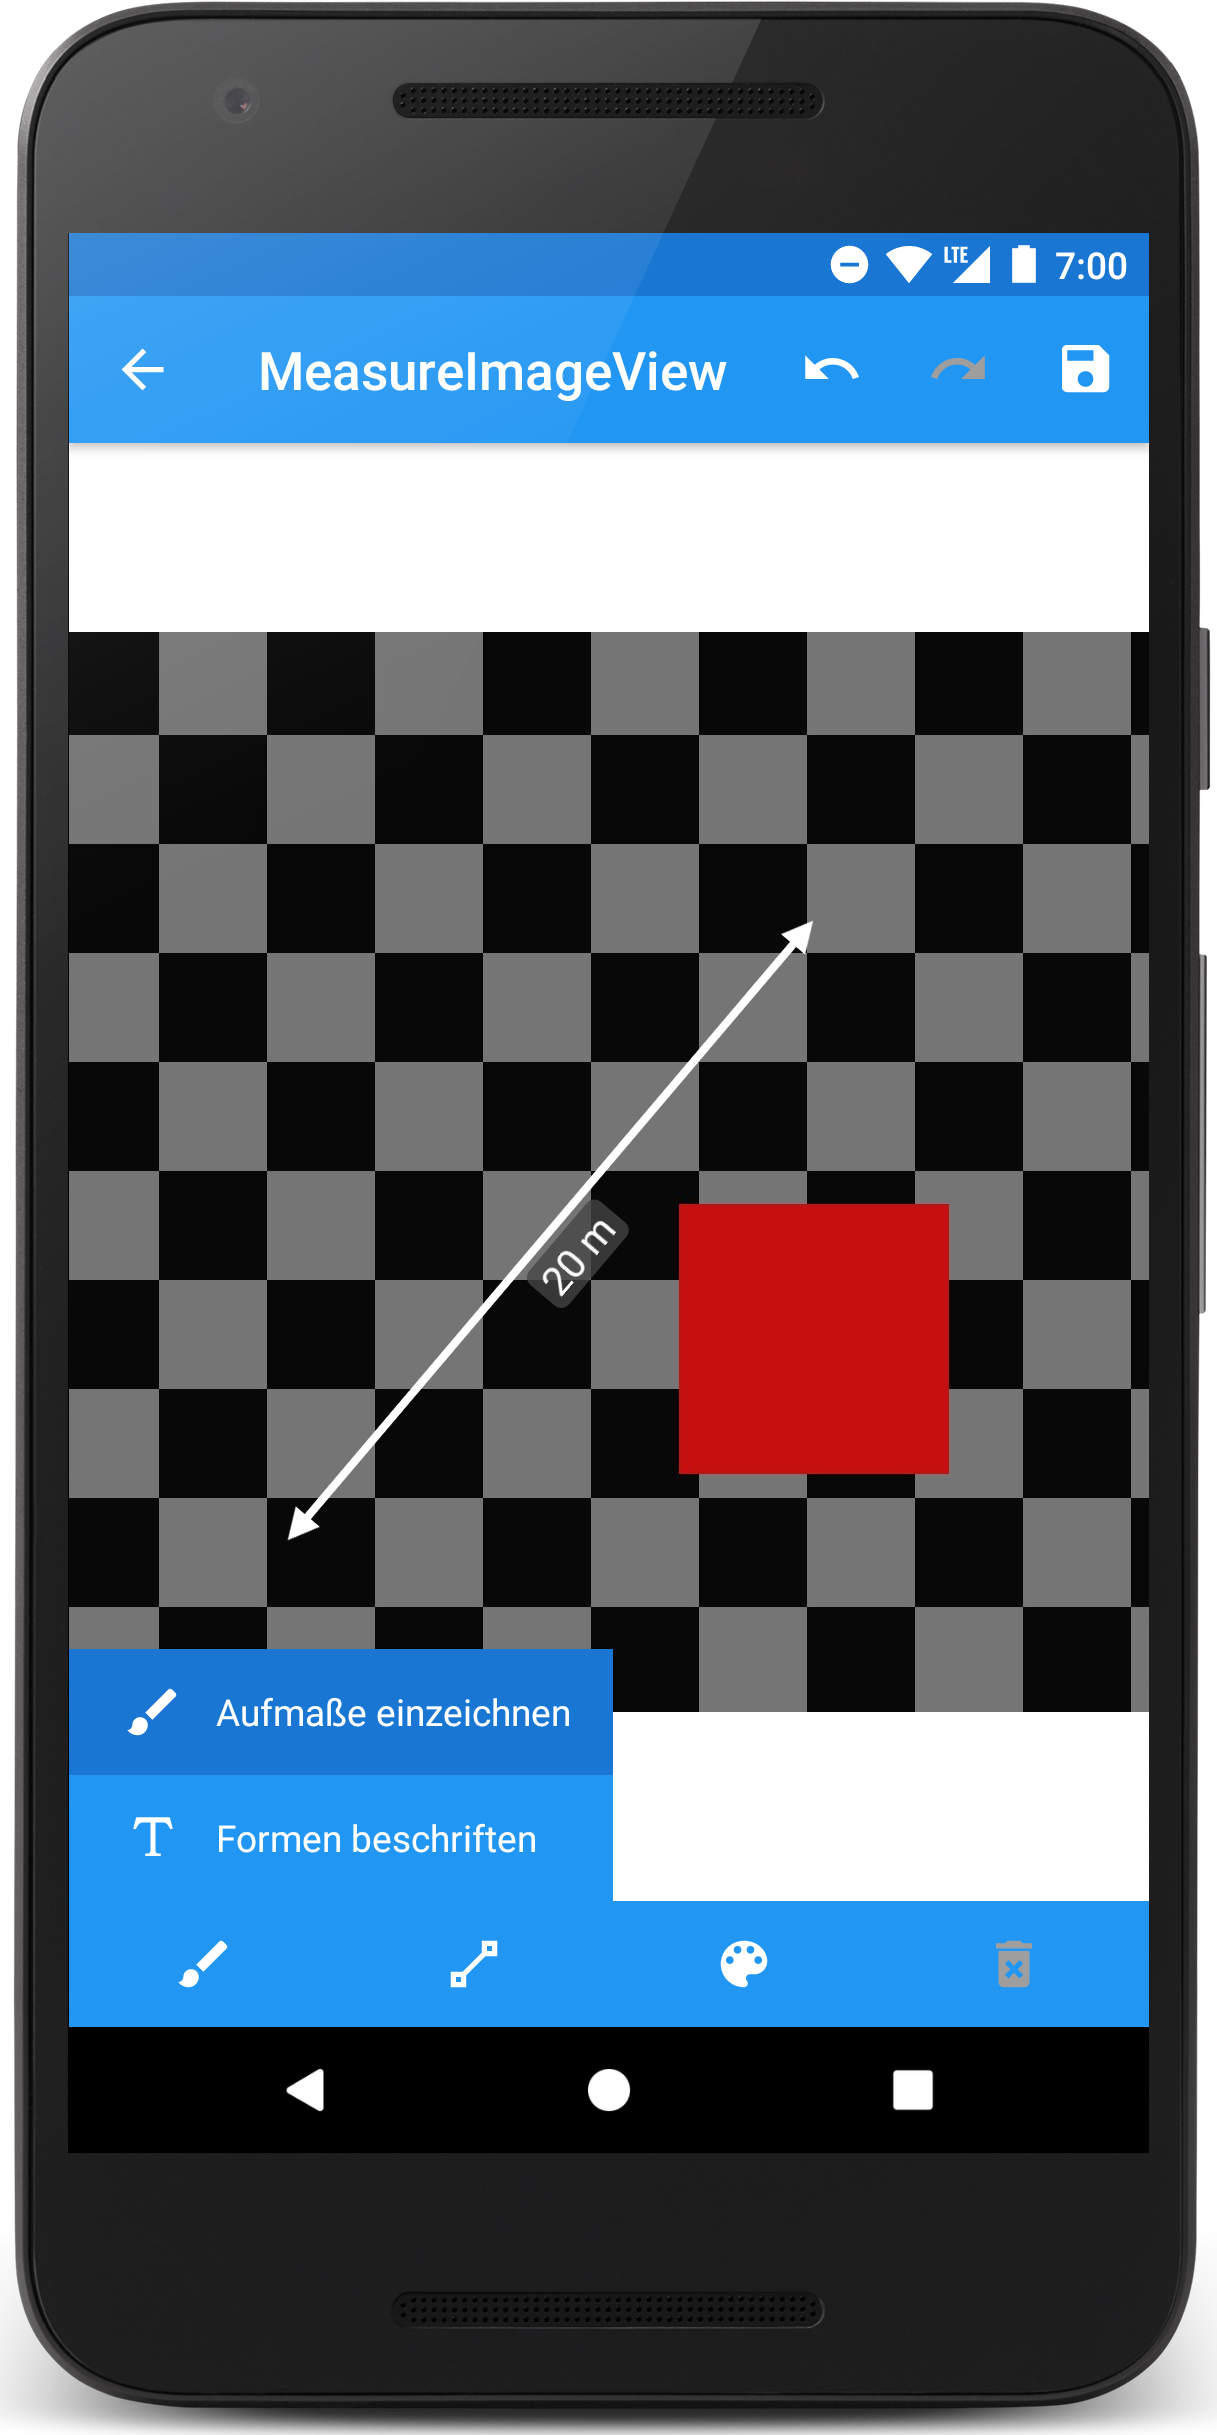
\includegraphics[keepaspectratio, width=\textwidth]{prototype2/expanded_mode}
    \caption{Statusleiste im Zeichen-Modus mit Popup-Dialog zur Auswahl des Modus}
    \label{fig:mode2}
  \end{subfigure}
  \begin{subfigure}[t]{0.4\textwidth}
    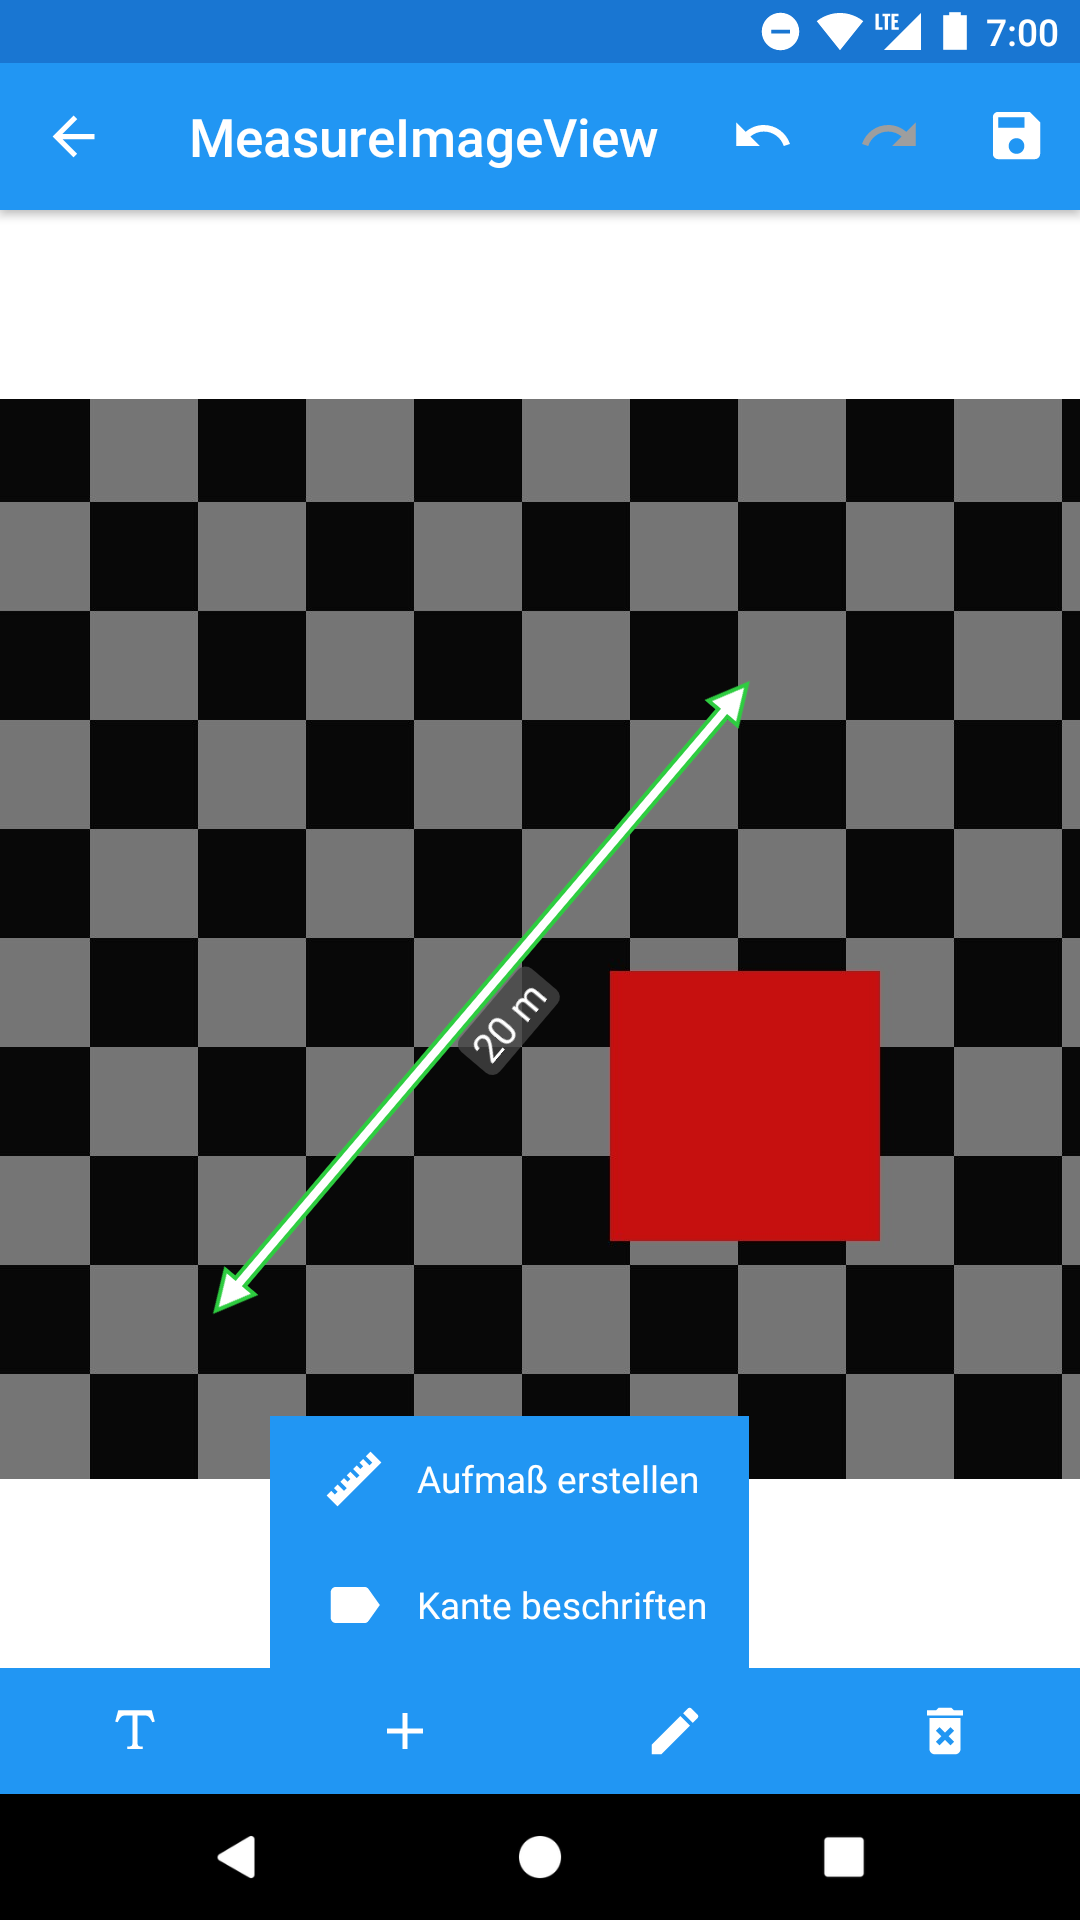
\includegraphics[keepaspectratio, width=\textwidth]{prototype2/label_popup}
    \caption{Statusleiste im Text-Modus mit Popup-Dialog zur Beschriftung der ausgewählten Form}
    \label{fig:labelp2}
  \end{subfigure}
  \centering
  \caption{Bedienung der Statusleiste im zweiten Prototyp}
  \label{fig:bar2}
\end{figure}

\noindent
Diese besteht aus vier verschiedenen Icons, die nur dann auswählbar sind, wenn die entsprechende Aktion im aktuellen Systemzustand legal durchführbar ist.
Das Icon ganz links ermöglicht das Wechseln zwischen dem Zeichen- und Text-Modus (siehe \autoref{fig:mode2}). \\

Im Zeichen-Modus kann per Klick auf das zweite Icon über ein \emph{Popup-Menü} die gewünschte Form ausgewählt werden. 
Im selben Modus kann beim Klick auf das dritte Icons (Farbpalette) die gewünschte Zeichenfarbe im Voraus konfiguriert werden. Hierzu öffnet sich, wie schon beim ersten Prototyp, ein modaler Farbauswahl-Dialog.
In beiden Modi ermöglicht das vierte Icon (Mülleimer) das Löschen der ausgewählten Form bzw. des markierten Textes. \\

Im Text-Modus kann beim Klick auf das zweite Icon über ein \emph{Popup-Menü} entweder eine ausgewählte Form mit einer Beschriftung versehen, oder mit einem Gerüsttyp verknüpft werden (siehe \autoref{fig:labelp2}).
Das dritte Icon ermöglicht das Bearbeiten von bereits eingetragenen Messwerten und verknüpften Gerüsttypen.
Auch in diesem Modus sind die Icons nur dann auswählbar, wenn der aktuelle Systemzustand dies zulässt. \\

Für eine einfache und fehlerfreie Benutzung auf Tablet-Geräten wurden sämtliche Größen mit Hilfe von dichteunabhängigen Pixeln modelliert, wie sie in den \emph{Android-Developer Guides} vorgeschlagen werden \citep{DP18}.
So werden hierbei alle Größen der Bildschirm-Elemente in der Einheit \emph{dp} (``density-independent pixel'') angegeben, welche zur Laufzeit vom System in normale Pixel (\emph{px}) umgewandelt werden.
Die genaue Umformung lautet dabei wie folgt:
\[
  px =  dp \times (\frac{dpi}{160}),
\]
wobei $dp$ für ``dots per inch'' steht.
Dies stellt sicher, dass, unabhängig von der Bilschirmgröße, alle Elemente ungefähr gleich groß dargestellt werden. \\
\todo{Bild vorher nachher Resize Points}

Messwerte sind mit einem grau-gefärbten Rechteck hinterlegt, welches dafür sorgt, dass sich der Text besser vom Hintergrund abhebt, und so auch bei dunkleren Bildern gut lesbar ist.
\todo{Bild vorher nachher}

Das Zuordnen von Gerüsttypen zu gezeichneten Formen wurde mit Hilfe eines modalen Dialogs umgesetzt, der neben dem Gerüsttyp auch noch Textfelder für die verschiedenen Dimensionen des Gerüsts besitzt.
Hierdurch kann der Benutzer nicht nur den Gerüsttyp, sondern auch Maße des Gerüsts, welche im Bild aufgrund des Aufnahmewinkels eventuell nicht zu sehen sind, eintragen und in den Meta-Daten speichern.
Formen zeigen mittels eines Indikators (siehe fig), mit wie vielen Gerüsttypen sie verbunden sind.
Auf diese Weise soll der Benutzer die bereits verlinkten von den nicht-verlinkten Formen unterscheiden können. \\
\todo{Bild von Dialog und Indikator}

Für das Schneiden und Rotieren von Bildern vor dem Annotieren wurde \emph{uCrop}, eine dedizierte Android-Library, welche auf \emph{Github} als Open-Source Projekt unter der \emph{Apache License Version 2.0} vorhanden ist, in das Projekt eingebunden \citep{UC18}.
Diese bietet im Gegensatz zu der \emph{Crop-Activity}, welche von manchen Android-Versionen zur Verfügung gestellt wird, Unterstützung für alle Gerätehersteller ab der Android-Version $14$ an.
\todo{Bilder lib}

\section{Testing}\label{sec:test2}
Der zweite Prototyp wurde sechs Tage, vom 3. bis zum 9. Januar 2018, von den beiden Geschäftsführern in den Arbeitsalltag integriert.
Das anschließende Feedback ergibt sich aus einem Gespräch am 9. Januar. \\

Als deutlich positive Verbesserung wurde dabei von beiden Testpersonen die neue Statusleiste am unteren Bildschirmrand genannt.
Hierdurch sei ihnen die Benutzung der App um einiges leichter gefallen, als noch beim ersten Prototyp mit den \emph{Floating Action Buttons}. \\

Jedoch sei, so beide Tester, das initiale Einarbeiten in die App immer noch zu schwierig, und nicht intuitiv genug.
Hier wünsche man sich ein ``kleines Bild, was die App kurz beschreibt'' (Testperson X) \\

Ein weiteres Problem, dass beim Testen des Prototyps aufgefallen ist, sei der Farbdialog.
Dieser sei nach Aussage von Testperson Y, zu fortgeschritten und biete eine Auswahl an Farben, die ``[...] der normale Gerüstbauer niemals verwendet wird'' \todo{Zitat hier?}
Dies ist ein Problem, welches während der Test-Phase zum ersten Prototyp nicht als solches identifiziert wurde, sich jetzt doch als ein solches herausgestellt hat.
Hierbei wäre es laut Testpersonen nämlich sinnvoller, den Benutzer ``[...] nicht mit so vielen Auswahlmöglichkeiten zu überfordern [...]'', sondern eine übersichtliche Menge an häufig benutzten Farben direkt auswählbar zu machen. \\

Außerdem wurde sich neben einem einfacheren Farbdialog eine Funktion gewünscht, Freitexte ins Bild einzutragen zu können. 
Dies sei laut der Aussage beider Testpersonen ein wichtiger Aspekt, da beim bisherigen Erstellen der Aufmaße oftmals weitere Notizen oder Kommentare auf den Skizzen eingetragen werden, um besondere Abmachungen bzw. Erkenntnisse festzuhalten. \\

Zudem fehle die Möglichkeit, Linien mit nur einer Pfeilspitze zu zeichnen.
Dies sei laut beider Testpersonen wichtig, um Längen, die auf dem Bild nur einen Startpunkt haben, und in die Tiefe offen sind, zu kennzeichnen. \\

Des Weiteren seien verlinkte Gerüsttypen an Formen nicht intuitiv durch den Indikator, wie er in dem ersten Prototyp umgesetzt wurde, erkennbar.
Zusätzlich wurde angemerkt, dass die Textfelder im Dialog zum Verlinken des Gerüsttyps durchaus sinnvoll seien, aber nur selten genutzt wurden, da sich Messwerte gemerkt werden müssen, um diese anschließend in den Dialog einzutragen. \\
